\documentclass[border=8pt]{standalone}
\usepackage{pgfplots}
\usepgfplotslibrary{colormaps}
\pgfplotsset{compat=1.18, trig format plots=rad}
\begin{document}
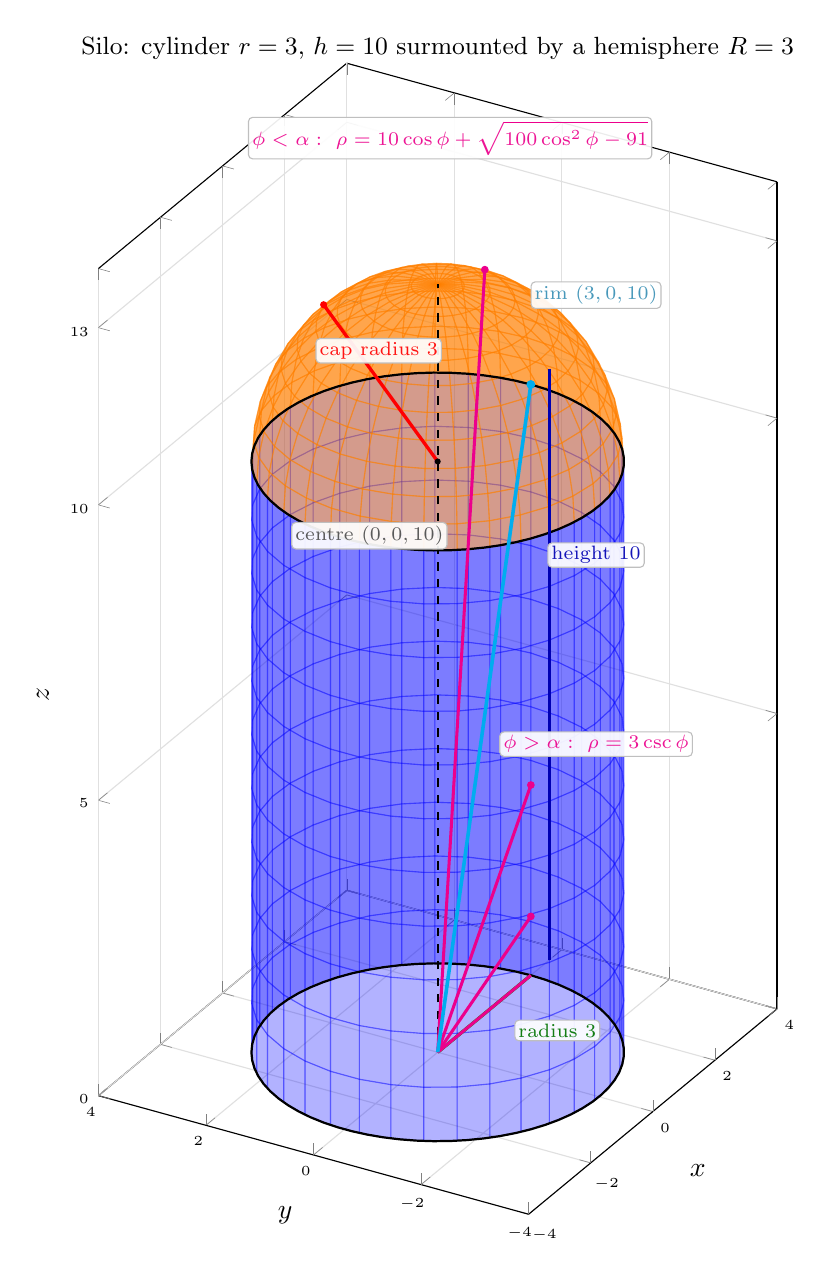
\begin{tikzpicture}
\begin{axis}[
    view={-60}{16},
    width=10.2cm, height=16.2cm,
    xlabel=$x$, ylabel=$y$, zlabel=$z$,
    xmin=-4,xmax=4, ymin=-4,ymax=4, zmin=0,zmax=14,
    xtick={-4,-2,...,4}, ytick={-4,-2,...,4}, ztick={0,5,10,13},
    every tick label/.append style={font=\tiny},
    grid=major, grid style={black!12},
    axis background/.style={fill=white},
    enlargelimits=false, clip=false,
    colormap/viridis high res,
]
% ---------- cylinder wall : r = 3, 0 <= z <= 10 ----------
\addplot3[surf, blue, opacity=0.30, shader=flat,
          domain=0:6.2832, y domain=0:10, samples=36, samples y=12]
   ({3*cos(x)}, {3*sin(x)}, {y});
% ---------- hemispherical cap : centre (0,0,10), R = 3 ----------
\addplot3[surf, orange, opacity=0.45, shader=flat,
          domain=0:6.2832, y domain=0:1.5708, samples=36, samples y=12]
   ({3*sin(y)*cos(x)}, {3*sin(y)*sin(x)}, {10+3*cos(y)});
% ---------- guide circles + axis of revolution ----------
\addplot3[thick, black, domain=0:6.2832, samples=70] ({3*cos(x)}, {3*sin(x)}, {0});
\addplot3[thick, black, domain=0:6.2832, samples=70] ({3*cos(x)}, {3*sin(x)}, {10});
\addplot3[dashed, thick, black] coordinates {(0,0,0) (0,0,13)};

% ---------- dimensions ----------
\addplot3[very thick, green!55!black] coordinates {(0,0,0) (3,0,0)};
\addplot3[very thick, blue!70!black] coordinates {(3.6,0,0) (3.6,0,10)};
\addplot3[very thick, red] coordinates {(0,0,10) (0,2.121,12.121)};
\fill[red] (axis cs:0,2.121,12.121) circle (1.3pt);
\fill[black] (axis cs:0,0,10) circle (1.1pt);

% ---------- spherical generating rays from the origin ----------
\addplot3[line width=1.1pt, magenta] coordinates {(0,0,0) (1.5178,0,12.5877)};
\addplot3[line width=1.1pt, magenta] coordinates {(0,0,0) (3,0,3.2203)};
\addplot3[line width=1.1pt, magenta] coordinates {(0,0,0) (3,0,0.9968)};
\addplot3[line width=1.1pt, magenta] coordinates {(0,0,0) (3,0,0)};
\addplot3[line width=1.3pt, cyan] coordinates {(0,0,0) (3,0,10)};
\fill[cyan]    (axis cs:3,0,10) circle (1.6pt);
\fill[magenta] (axis cs:1.5178,0,12.5877) circle (1.4pt);
\fill[magenta] (axis cs:3,0,3.2203) circle (1.4pt);
\fill[magenta] (axis cs:3,0,0.9968) circle (1.4pt);

% ---------- labels (white backing keeps them readable over the meshes) ----------
\tikzset{lbl/.style={font=\scriptsize,inner sep=1.3pt,rounded corners=1.5pt,
                     fill=white,fill opacity=0.92,draw=black!25}}
\node[lbl,text=green!45!black] at (axis cs:1.6,-1.3,0) {radius $3$};
\node[lbl,text=blue!70!black] at (axis cs:5.1,0,6.2) {height $10$};
\node[lbl,text=red] at (axis cs:-1.9,0,12.7) {cap radius $3$};
\node[lbl,text=black!70] at (axis cs:-2.2,0,9.7) {centre $(0,0,10)$};
\node[lbl,text=cyan!70!black] at (axis cs:5.1,0,10.6) {rim $(3,0,10)$};
\node[lbl,text=magenta] at (axis cs:5.1,0,3.0) {$\phi>\alpha:\ \rho=3\csc\phi$};
\node[lbl,text=magenta,align=left] at (axis cs:0.4,0,15.3)
   {$\phi<\alpha:\ \rho=10\cos\phi+\sqrt{100\cos^2\phi-91}$};
\node[font=\small,text=black] at (axis cs:0,0,17.0)
   {Silo: cylinder $r=3$, $h=10$ surmounted by a hemisphere $R=3$};
\end{axis}
\end{tikzpicture}
\end{document}
